% =============================================================================
%  Trabalho Prático I - Fundamentos de Inteligência Artificial (UFMG / DEE)
%  O Problema da Ponte e da Tocha como busca em espaço de estados
%
%  Compilar com pdfLaTeX (Overleaf: "Compiler: pdfLaTeX", arquivo principal
%  main.tex). Bibliografia em referencias.bib, estilo apalike (formato APA).
%
%  Os comentários "% TODO grupo:" marcam a prosa que o grupo escreve. Tabelas,
%  figuras e definições formais já estão preenchidas com os números gerados
%  por `make report` e `make charts` (ver resultados.md).
% =============================================================================
\documentclass[12pt,a4paper]{article}

\usepackage[utf8]{inputenc}
\usepackage[T1]{fontenc}
\usepackage{lmodern}
\usepackage[brazil]{babel}
\usepackage[a4paper,margin=2.5cm]{geometry}
\usepackage{amsmath,amssymb}
\usepackage{graphicx}
\usepackage{booktabs}
\usepackage{multirow}
\usepackage{caption}
\usepackage{float}
\usepackage{algorithm}
\usepackage{algpseudocode}
\usepackage{natbib}
\usepackage[hidelinks]{hyperref}

\graphicspath{{figuras/}}

% Nomes em português para os ambientes de algoritmo.
\floatname{algorithm}{Algoritmo}
\renewcommand{\listalgorithmname}{Lista de Algoritmos}
\algrenewcommand\algorithmicrequire{\textbf{Entrada:}}
\algrenewcommand\algorithmicensure{\textbf{Saída:}}

% Atalhos de notação usados ao longo do texto.
\newcommand{\cost}{\operatorname{custo}}
\newcommand{\Esq}{E}
\newcommand{\Dir}{D}
\newcommand{\state}[3]{\langle #1,\ #2,\ #3\rangle}

\title{\textbf{O Problema da Ponte e da Tocha\\como Busca em Espaço de Estados}\\[0.5em]
       \large Trabalho Prático I -- Fundamentos de Inteligência Artificial}
\author{Arthur Fernandes \and Bruno Lima \and Felipe Augusto
        % TODO grupo: o enunciado exige grupos de 4 integrantes. Incluir o 4º nome.
        }
\date{Universidade Federal de Minas Gerais -- Departamento de Engenharia Elétrica\\
      Profs. Cristiano Castro e João Pedro Campos\\[0.5em]
      \today}

\begin{document}

\maketitle

\begin{abstract}
% TODO grupo: resumo de um parágrafo (5-8 linhas): o problema, a modelagem como
% grafo de espaço de estados, os quatro métodos implementados, o principal
% resultado (solução ótima de 17 minutos, encontrada por Custo Mínimo e A*;
% BFS e DFS devolvem 19 minutos) e a conclusão sobre as heurísticas.
\end{abstract}

\tableofcontents
\newpage

% -----------------------------------------------------------------------------
\section{Introdução}
\label{sec:introducao}
% TODO grupo:
%  - Apresentar o quebra-cabeça (4 pessoas: 1, 2, 5 e 10 min; ponte para 2;
%    tocha obrigatória; velocidade do mais lento) e o objetivo (tempo mínimo).
%  - Dizer por que ele é um bom exemplo de busca em espaço de estados: espaço
%    pequeno o bastante para ser desenhado por inteiro, mas com custos de aresta
%    não uniformes - o que separa os métodos cegos dos métodos de custo.
%  - Enumerar as quatro tarefas do enunciado e como o relatório está organizado
%    (Seções \ref{sec:modelagem} a \ref{sec:conclusao}).
%  - Mencionar que todo o código, os testes e o relatório gerado
%    automaticamente estão no repositório do grupo.

% -----------------------------------------------------------------------------
\section{Modelagem do problema}
\label{sec:modelagem}

\subsection{Representação de estado}
\label{sec:estado}

Um estado é uma tripla
\begin{equation}
  s = \state{\Esq}{\Dir}{t},
  \qquad \Esq \cup \Dir = P,\quad \Esq \cap \Dir = \emptyset,\quad t \in \{\text{esq},\ \text{dir}\},
  \label{eq:estado}
\end{equation}
em que $P = \{p_1, p_2, p_5, p_{10}\}$ é o conjunto de pessoas (cada uma com o seu tempo de travessia $\tau(p)$), $\Esq$ e $\Dir$ são as pessoas na margem esquerda e na margem direita, e $t$ é o lado em que está a tocha. Ao longo do texto, um estado é escrito de forma compacta como \texttt{*[1, 2] \textasciitilde{}\textasciitilde{}\textasciitilde{} [5, 10]}: o asterisco marca o lado da tocha e \texttt{-} indica uma margem vazia.

% TODO grupo:
%  - Explicar por que a tripla captura toda a informação necessária (posição de
%    cada pessoa + posição da tocha) e por que a tocha precisa fazer parte do
%    estado (sem ela, dois estados com as mesmas pessoas de cada lado seriam
%    indistinguíveis, mas admitem ações diferentes).
%  - Comentar que a identidade da pessoa é separada do seu tempo: duas pessoas
%    igualmente rápidas continuam sendo duas pessoas (classe Person, com id e
%    time). Como D é o complemento de E, bastaria guardar E e t; o código guarda
%    os dois lados por legibilidade.
%  - Notar que há 2^4 x 2 = 32 configurações concebíveis, das quais apenas 30
%    são alcançáveis (Seção \ref{sec:grafo}).

\subsection{Estado inicial e estado objetivo}
\label{sec:inicial-objetivo}

\begin{align}
  s_0 &= \state{\{p_1,p_2,p_5,p_{10}\}}{\emptyset}{\text{esq}}
       &&\text{(\texttt{*[1, 2, 5, 10] \textasciitilde\textasciitilde\textasciitilde{} [-]})}, \label{eq:inicial}\\
  s_\star &= \state{\emptyset}{\{p_1,p_2,p_5,p_{10}\}}{\text{dir}}
       &&\text{(\texttt{[-] \textasciitilde\textasciitilde\textasciitilde{} [1, 2, 5, 10]*})}. \label{eq:objetivo}
\end{align}

% TODO grupo: uma ou duas frases: o teste de objetivo é "margem esquerda vazia
% e tocha à direita"; há um único estado objetivo.

\subsection{Ações, função sucessora, transições e custos}
\label{sec:sucessora}

Em um estado $s = \state{\Esq}{\Dir}{t}$, seja $L(s)$ o conjunto de pessoas do lado da tocha ($L(s)=\Esq$ se $t=\text{esq}$, $L(s)=\Dir$ caso contrário). Uma \emph{ação} é um grupo $g \subseteq L(s)$ com $1 \le |g| \le 2$ que atravessa a ponte levando a tocha. A função sucessora devolve, para cada ação válida, o estado resultante e o custo da transição:
\begin{equation}
  \operatorname{suc}(s) = \bigl\{\, (g,\ s',\ \cost(g)) \ :\ g \subseteq L(s),\ 1 \le |g| \le 2 \,\bigr\},
  \qquad
  \cost(g) = \max_{p \in g} \tau(p),
  \label{eq:sucessora}
\end{equation}
em que $s'$ é obtido movendo $g$ para a outra margem e trocando o lado da tocha. Assim, para $t=\text{esq}$, $s' = \state{\Esq \setminus g}{\Dir \cup g}{\text{dir}}$; para $t=\text{dir}$, $s' = \state{\Esq \cup g}{\Dir \setminus g}{\text{esq}}$.

O custo de um caminho $\langle s_0, s_1, \ldots, s_k\rangle$ é a soma dos custos das suas transições, isto é, o tempo total de travessia acumulado:
\begin{equation}
  g(s_k) = \sum_{i=1}^{k} \cost(g_i).
  \label{eq:g}
\end{equation}

% TODO grupo:
%  - Explicar em palavras: quem pode agir é quem está com a tocha; grupos de
%    1 ou 2 pessoas (capacidade da ponte); o custo é o tempo do mais lento.
%  - Dar o número de ações em cada situação: com m pessoas do lado da tocha há
%    m + C(m,2) ações (10 no estado inicial: 4 individuais + 6 pares; 3 quando
%    duas pessoas estão com a tocha; 1 quando só uma).
%  - Observar que toda travessia é reversível (o mesmo grupo pode voltar), o
%    que torna o grafo simétrico e cheio de ciclos - isso justifica a poda de
%    estados repetidos usada em todos os algoritmos (Seção \ref{sec:algoritmos}).
%  - Mencionar que tempos e capacidade são parâmetros (BridgeProblem(times,
%    capacity)), usados no experimento de escalabilidade.

\subsection{O grafo do espaço de estados}
\label{sec:grafo}

\begin{figure}[H]
  \centering
  
\includegraphics[width=\textwidth]{bridge_state_graph.png}
  \caption{Grafo do espaço de estados: 30 estados alcançáveis dispostos em camadas pelo número de pessoas já na margem direita, e 112 transições dirigidas. Em vermelho, o caminho de custo mínimo (17 minutos); o quadro à esquerda lista as suas travessias. Gerado por \texttt{make graph}.}
  \label{fig:grafo}
\end{figure}

\begin{table}[H]
  \centering
  \caption{Propriedades do grafo de espaço de estados da instância do enunciado.}
  \label{tab:grafo}
  \begin{tabular}{lr}
    \toprule
    Métrica & Valor \\
    \midrule
    Pessoas & 4 \\
    Configurações concebíveis ($2^4 \times 2$) & 32 \\
    Estados alcançáveis ($|V|$) & 30 \\
    Transições dirigidas ($|E|$) & 112 \\
    Grau de saída (mín. / médio / máx.) & 1 / 3,73 / 10 \\
    Posições de uma matriz de adjacências ($|V|^2$) & 900 \\
    Densidade ($|E| / |V|^2$) & 12,4\,\% \\
    \bottomrule
  \end{tabular}
\end{table}

\begin{table}[H]
  \centering
  \caption{Trecho da lista de adjacências: as transições que partem do estado inicial (\texttt{E00}) e de um estado intermediário (\texttt{E09}). A lista completa, com os 30 estados, está em \texttt{resultados.md}.}
  \label{tab:adjacencia}
  \small
  \begin{tabular}{llcrl}
    \toprule
    Estado de origem & Ação & Sentido & Custo (min) & Estado resultante \\
    \midrule
    \multirow{10}{*}{\texttt{E00} \texttt{*[1, 2, 5, 10] \textasciitilde\textasciitilde\textasciitilde{} [-]}}
      & \{1\}     & $\rightarrow$ &  1 & \texttt{E08} \texttt{[2, 5, 10] \textasciitilde\textasciitilde\textasciitilde{} [1]*} \\
      & \{1, 2\}  & $\rightarrow$ &  2 & \texttt{E20} \texttt{[5, 10] \textasciitilde\textasciitilde\textasciitilde{} [1, 2]*} \\
      & \{2\}     & $\rightarrow$ &  2 & \texttt{E07} \texttt{[1, 5, 10] \textasciitilde\textasciitilde\textasciitilde{} [2]*} \\
      & \{1, 5\}  & $\rightarrow$ &  5 & \texttt{E19} \texttt{[2, 10] \textasciitilde\textasciitilde\textasciitilde{} [1, 5]*} \\
      & \{2, 5\}  & $\rightarrow$ &  5 & \texttt{E17} \texttt{[1, 10] \textasciitilde\textasciitilde\textasciitilde{} [2, 5]*} \\
      & \{5\}     & $\rightarrow$ &  5 & \texttt{E06} \texttt{[1, 2, 10] \textasciitilde\textasciitilde\textasciitilde{} [5]*} \\
      & \{1, 10\} & $\rightarrow$ & 10 & \texttt{E18} \texttt{[2, 5] \textasciitilde\textasciitilde\textasciitilde{} [1, 10]*} \\
      & \{2, 10\} & $\rightarrow$ & 10 & \texttt{E16} \texttt{[1, 5] \textasciitilde\textasciitilde\textasciitilde{} [2, 10]*} \\
      & \{5, 10\} & $\rightarrow$ & 10 & \texttt{E15} \texttt{[1, 2] \textasciitilde\textasciitilde\textasciitilde{} [5, 10]*} \\
      & \{10\}    & $\rightarrow$ & 10 & \texttt{E05} \texttt{[1, 2, 5] \textasciitilde\textasciitilde\textasciitilde{} [10]*} \\
    \midrule
    \multirow{3}{*}{\texttt{E09} \texttt{*[1, 2] \textasciitilde\textasciitilde\textasciitilde{} [5, 10]}}
      & \{1\}     & $\rightarrow$ &  1 & \texttt{E26} \texttt{[2] \textasciitilde\textasciitilde\textasciitilde{} [1, 5, 10]*} \\
      & \{1, 2\}  & $\rightarrow$ &  2 & \texttt{E29} \texttt{[-] \textasciitilde\textasciitilde\textasciitilde{} [1, 2, 5, 10]*} \\
      & \{2\}     & $\rightarrow$ &  2 & \texttt{E25} \texttt{[1] \textasciitilde\textasciitilde\textasciitilde{} [2, 5, 10]*} \\
    \bottomrule
  \end{tabular}
\end{table}

% TODO grupo (explicação da modelagem na forma de grafo - item obrigatório):
%  - Vértices = estados, arestas dirigidas = transições rotuladas pela ação e
%    pelo custo; referenciar a Figura \ref{fig:grafo} e a Tabela \ref{tab:grafo}.
%  - Por que 2 configurações são inalcançáveis (tocha acompanha quem atravessa:
%    ninguém pode estar todo de um lado com a tocha do outro).
%  - O grafo é simétrico (toda aresta tem a inversa com o mesmo custo): 112
%    arestas dirigidas = 56 não dirigidas; consequência: ciclos.
%  - Lista de adjacências vs. matriz: a matriz teria 900 posições com apenas
%    112 não nulas (12,4%); a lista guarda só os vizinhos reais e é gerada sob
%    demanda pela função sucessora. Referenciar a Tabela \ref{tab:adjacencia}.
%  - Organização em camadas (número de pessoas já à direita): idas avançam uma
%    camada, voltas recuam.

% -----------------------------------------------------------------------------
\section{Algoritmos de busca}
\label{sec:algoritmos}

\subsection{Procedimento geral de busca}
\label{sec:procedimento-geral}

Todos os métodos implementados são instâncias do mesmo procedimento (Algoritmo~\ref{alg:busca}), no qual a \emph{fronteira} é um conjunto de caminhos que partem do estado inicial. O que distingue uma estratégia da outra é apenas o critério de escolha do próximo caminho a ser removido da fronteira \citep{poole2017}.

\begin{algorithm}[H]
  \caption{Procedimento geral de busca em grafo com poda de estados repetidos.}
  \label{alg:busca}
  \begin{algorithmic}[1]
    \Require estado inicial $s_0$, função sucessora $\operatorname{suc}$, teste de objetivo, limite $N_{\max}$ de expansões
    \Ensure um caminho de $s_0$ até um estado objetivo, ou falha
    \State fronteira $\gets \{\langle s_0\rangle\}$;\quad explorados $\gets \emptyset$;\quad expandidos $\gets 0$
    \While{fronteira $\neq \emptyset$}
      \If{expandidos $\ge N_{\max}$} \Return falha (limite atingido) \EndIf
      \State selecionar e remover um caminho $\langle s_0,\ldots,s_k\rangle$ da fronteira \Comment{critério da estratégia}
      \If{$s_k$ é objetivo} \Return $\langle s_0,\ldots,s_k\rangle$ \EndIf
      \State explorados $\gets$ explorados $\cup\ \{s_k\}$;\quad expandidos $\gets$ expandidos $+ 1$
      \ForAll{$(g, s', c) \in \operatorname{suc}(s_k)$}
        \If{$s'$ não foi podado} \Comment{já explorado ou já na fronteira com custo menor ou igual}
          \State adicionar $\langle s_0,\ldots,s_k,s'\rangle$ à fronteira
        \EndIf
      \EndFor
    \EndWhile
    \State \Return falha
  \end{algorithmic}
\end{algorithm}

% TODO grupo:
%  - Explicar o algoritmo em palavras: fronteira, expansão, teste de objetivo
%    no momento da remoção (e não na geração), poda de estados repetidos.
%  - Justificar o limite N_max (recomendação do enunciado; padrão 15 000
%    expansões, parametrizável por --max-expansoes) e por que ele importa para
%    o DFS.
%  - Dizer o que é medido em cada execução: nós expandidos (caminhos removidos
%    da fronteira e expandidos; o objetivo não conta), nós gerados, tamanho
%    máximo da fronteira e tempo de processamento.

\subsection{Busca em largura (BFS)}
\label{sec:bfs}
% TODO grupo (explicação básica - item obrigatório):
%  - Fronteira em fila FIFO: seleciona o caminho com menos arestas.
%  - Completa; ótima apenas quando todas as arestas têm o mesmo custo
%    (\citealp{russell2021}). Aqui os custos variam de 1 a 10.
%  - Poda: um estado já explorado ou já presente na fronteira não é
%    reinserido, mesmo que o novo caminho até ele seja mais barato - é isso
%    que faz a BFS devolver 19 minutos (Seção \ref{sec:por-que-bfs}).

\subsection{Busca em profundidade (DFS)}
\label{sec:dfs}
% TODO grupo:
%  - Fronteira em pilha LIFO: aprofunda um ramo antes de considerar
%    alternativas. Os sucessores são empilhados em ordem inversa para serem
%    desempilhados na ordem em que a função sucessora os gera (mais rápidos
%    primeiro).
%  - Sem poda de repetidos, ficaria indo e voltando pela ponte para sempre
%    (o grafo tem ciclos); com a poda e um grafo finito, termina.
%  - Não é ótima nem, em geral, completa; o limite de expansões é a garantia
%    prática de término.

\subsection{Busca de custo mínimo (custo uniforme)}
\label{sec:lcfs}
% TODO grupo:
%  - Fronteira em fila de prioridade ordenada por g(n) (Eq. \ref{eq:g}):
%    seleciona sempre o caminho de menor custo acumulado.
%  - Equivale ao algoritmo de Dijkstra \citep{dijkstra1959} com teste de
%    objetivo na remoção; como todo custo de aresta é positivo, o primeiro
%    caminho até o objetivo a ser removido é ótimo.
%  - Implementação: heap binário (heapq); guarda-se o melhor custo já
%    enfileirado por estado para não empilhar caminhos dominados.

\subsection{Busca A*}
\label{sec:astar}
% TODO grupo:
%  - Fronteira ordenada por f(n) = g(n) + h(n) \citep{hart1968}.
%  - Com h admissível, a solução devolvida é ótima; com h consistente, nenhum
%    estado precisa ser reexpandido.
%  - Diferença para a busca de custo mínimo: só a chave de ordenação muda
%    (ver o código: AStarSearch e LowestCostFirstSearch diferem apenas na
%    prioridade).

\subsection{Função de custo e heurísticas}
\label{sec:heuristicas}

A função de custo $g(n)$ é a da Equação~\eqref{eq:g}: o tempo total acumulado até o estado $n$. Foram propostas duas heurísticas, ambas admissíveis e consistentes.

\paragraph{Heurística $h_1$.} Tempo da pessoa mais lenta que ainda está na margem esquerda:
\begin{equation}
  h_1(s) = \begin{cases}
    \max_{p \in \Esq} \tau(p), & \Esq \neq \emptyset,\\
    0, & \Esq = \emptyset.
  \end{cases}
  \label{eq:h1}
\end{equation}

% TODO grupo (justificativa de admissibilidade - item obrigatório):
%  - Toda pessoa à esquerda ainda precisa atravessar; a mais lenta delas fará
%    ao menos uma ida, e essa ida custa pelo menos o tempo dela. Logo h1 <= h*.
%  - Consistência: ao mover um grupo g, h1 cai no máximo max_{p in g} tau(p)
%    = custo da aresta (se o mais lento sai da esquerda) ou não muda/cresce.

\paragraph{Heurística $h_2$.} Sejam $t_1 \ge t_2 \ge \cdots \ge t_m$ os tempos das $m$ pessoas ainda na margem esquerda, $c$ a capacidade da ponte ($c = 2$ na instância do enunciado) e $\tau_{\min}$ o tempo da pessoa mais rápida do problema. Então
\begin{equation}
  h_2(s) = \underbrace{\sum_{i \,\equiv\, 1 \ (\mathrm{mod}\ c)} t_i}_{\text{idas}}
         \;+\;
         \underbrace{r(s)\,\tau_{\min}}_{\text{voltas}},
  \qquad
  r(s) = \begin{cases}
    \lceil m/c \rceil - 1, & t = \text{esq},\\
    \lceil m/c \rceil,     & t = \text{dir},
  \end{cases}
  \label{eq:h2}
\end{equation}
com $h_2(s) = 0$ quando $\Esq = \emptyset$. Para $c=2$, a parcela das idas é $t_1 + t_3 + t_5 + \cdots$.

% TODO grupo (justificativa de admissibilidade):
%  - Idas: cada pessoa à esquerda tem uma última travessia de ida; isso
%    particiona as m pessoas em grupos de até c, logo há pelo menos ceil(m/c)
%    idas. Os i grupos mais caros cobrem no máximo i*c pessoas, então o i-ésimo
%    maior custo de ida é >= t_{(i-1)c+1}. A soma t_1 + t_{c+1} + ... é um
%    limite inferior (com c=2: emparelhar 10 com 5 e 2 com 1 dá 10 + 2 = 12).
%  - Voltas: entre duas idas consecutivas alguém traz a tocha de volta; são
%    pelo menos ceil(m/c) - 1 voltas (ou ceil(m/c) se a tocha está à direita),
%    cada uma custando no mínimo tau_min. No estado inicial: 12 + 1 = 13.
%  - h2 >= h1 em todo estado (t_1 é o primeiro termo), logo h2 domina h1.
%  - As duas propriedades foram verificadas exaustivamente nos 30 estados e
%    112 transições (Tabela \ref{tab:heuristicas}) - e também em instâncias com
%    5 pessoas e capacidade 3, pela suíte de testes.

\begin{table}[H]
  \centering
  \caption{Comparação das heurísticas na instância do enunciado. $h^\ast$ é o custo real até o objetivo, obtido por busca de custo mínimo sobre o grafo invertido; a verificação de admissibilidade e consistência é exaustiva sobre os 30 estados e as 112 transições.}
  \label{tab:heuristicas}
  \begin{tabular}{lrrccrrr}
    \toprule
    Heurística & $h(s_0)$ & $h^\ast(s_0)$ & Admissível & Consistente & Erro médio $h^\ast\!-\!h$ & Nós exp. (A*) & Custo \\
    \midrule
    $h_1$ & 10 & 17 & sim & sim & 3,70 & 18 & 17 \\
    $h_2$ & 13 & 17 & sim & sim & 2,53 & 14 & 17 \\
    \bottomrule
  \end{tabular}
\end{table}

% -----------------------------------------------------------------------------
\section{Implementação}
\label{sec:implementacao}
% TODO grupo (explicação clara das rotinas desenvolvidas - item obrigatório):
%  - Linguagem e organização: Python 3, pacote src/ com models/ (Person, State,
%    Arc, Path, BridgeProblem), algorithms/ (BaseSearch, BreadthFirstSearch,
%    DepthFirstSearch, LowestCostFirstSearch, AStarSearch) e utils/
%    (heurísticas, espaço de estados, relatórios, escalabilidade, gráficos).
%  - Person/State: dataclasses imutáveis (frozenset), hashable, para servirem
%    de chave nos conjuntos de explorados.
%  - Arc e Path: a fronteira guarda caminhos; Path é definido recursivamente
%    (nó inicial, ou caminho seguido de um arco), então estender custa O(1) e
%    caminhos com prefixo comum compartilham memória.
%  - BridgeProblem.get_successors: gera as combinações de 1..capacity pessoas
%    do lado da tocha (itertools.combinations), memoizada porque é
%    determinística; o cache é aquecido antes das medições para que todos os
%    métodos sejam cronometrados nas mesmas condições.
%  - BaseSearch: contadores compartilhados (expandidos, gerados, fronteira
%    máxima), limite de expansões, run_once (perf_counter, em µs) e execute
%    (N repetições -> média, desvio, mínimo).
%  - CLI (python -m src.main): --algoritmos, --repeticoes, --tempos,
%    --capacidade, --max-expansoes, --sem-cache, --saida.
%  - Testes: pytest, 76 testes (modelagem, algoritmos, métricas, heurísticas
%    em 4 instâncias, grafo, CLI, escalabilidade, gráficos).
%  - Relatório automático (resultados.md) em seções idempotentes e figura do
%    grafo com networkx/matplotlib.

% -----------------------------------------------------------------------------
\section{Resultados e discussão}
\label{sec:resultados}

\subsection{Comparação dos métodos na instância do enunciado}
\label{sec:comparacao}

\begin{table}[H]
  \centering
  \caption{Comparação dos métodos na instância do enunciado (tempos 1, 2, 5 e 10; ponte para duas pessoas). Cada método foi executado 1000 vezes: custo, número de travessias, nós expandidos, nós gerados e fronteira máxima são determinísticos e idênticos em todas as repetições; o tempo de processamento é a média e o desvio-padrão das repetições, medido com \texttt{time.perf\_counter()}. Máquina: \emph{[processador, sistema operacional e versão do Python]}.}
  % TODO grupo: substituir o trecho entre colchetes pela máquina usada na medição.
  \label{tab:comparacao}
  \small
  \begin{tabular}{lrrrrrr}
    \toprule
    Método & Custo (min) & Travessias & Nós exp. & Nós ger. & Front. máx. & Tempo (µs) \\
    \midrule
    Busca em largura (BFS)       & 19 & 5 & 25 & 98 & 10 & $50{,}4 \pm 20{,}3$ \\
    Busca em profundidade (DFS)  & 19 & 5 &  9 & 32 & 12 & $20{,}1 \pm 4{,}8$ \\
    Busca de custo mínimo        & \textbf{17} & 5 & 25 & 98 & 11 & $59{,}7 \pm 7{,}5$ \\
    A* com $h_1$                 & \textbf{17} & 5 & 18 & 71 & 14 & $55{,}0 \pm 5{,}4$ \\
    A* com $h_2$                 & \textbf{17} & 5 & 14 & 57 & 14 & $59{,}6 \pm 32{,}5$ \\
    \bottomrule
  \end{tabular}
\end{table}

\begin{table}[H]
  \centering
  \caption{Caminhos devolvidos por cada método. BFS e DFS devolvem o mesmo caminho de 19 minutos; busca de custo mínimo e A* (com $h_1$ e com $h_2$) devolvem o caminho ótimo de 17 minutos.}
  \label{tab:caminhos}
  \begin{tabular}{lll}
    \toprule
    Passo & BFS e DFS (19 min) & Custo mínimo e A* (17 min) \\
    \midrule
    1 & ida \{1, 2\} (2 min)   & ida \{1, 2\} (2 min) \\
    2 & volta \{1\} (1 min)    & volta \{1\} (1 min) \\
    3 & ida \{1, 5\} (5 min)   & ida \{5, 10\} (10 min) \\
    4 & volta \{1\} (1 min)    & volta \{2\} (2 min) \\
    5 & ida \{1, 10\} (10 min) & ida \{1, 2\} (2 min) \\
    \bottomrule
  \end{tabular}
\end{table}

% TODO grupo:
%  - Ler a Tabela \ref{tab:comparacao} linha a linha: custo, nós expandidos e
%    tempo. Destacar que os três métodos de custo chegam a 17 e os dois cegos
%    a 19; que A*(h2) expande 14 nós contra 25 da busca de custo mínimo
%    (44% a menos) e 18 de A*(h1).
%  - Explicar por que o enunciado pede "valores médios": custo e nós
%    expandidos são determinísticos (a função sucessora é determinística e os
%    desempates são fixos), então a média só faz sentido para o tempo, que
%    varia com o sistema operacional; por isso 1000 repetições e o desvio.
%  - Comentar os tempos: na instância de 4 pessoas todos terminam em dezenas
%    de microssegundos e o DFS é o mais rápido justamente porque para no
%    primeiro ramo que encontra o objetivo; a ordem entre os outros é
%    dominada pelo custo por nó (heap + heurística) e não pelo número de nós.
%  - Comentar a solução ótima (Tabela \ref{tab:caminhos}): a ideia-chave é
%    fazer os dois mais lentos atravessarem juntos, usando os dois mais
%    rápidos como "portadores" da tocha.

\subsection{Por que a busca em largura não garante a solução ótima}
\label{sec:por-que-bfs}
% TODO grupo (item obrigatório do enunciado):
%  - A BFS minimiza o número de arestas do caminho, não o seu custo. Ela só é
%    ótima quando o custo é uma função não decrescente da profundidade - por
%    exemplo, quando todas as arestas custam o mesmo \citep{russell2021}.
%  - Aqui as arestas custam de 1 a 10. O caminho ótimo e o caminho da BFS têm
%    ambos 5 travessias (Tabela \ref{tab:caminhos}); entre todos os caminhos
%    de 5 arestas, a BFS devolve o primeiro que alcança o objetivo na ordem em
%    que os estados foram gerados, e não o mais barato.
%  - Detalhe mecânico: quando um estado já está na fronteira, a BFS descarta
%    qualquer novo caminho até ele - mesmo mais barato. O estado
%    *[1, 2] ~~~ [5, 10] (E09) é alcançado primeiro pelo caminho {1,2}->,
%    {1}<-, {1,5}->, {1}<- ... (via 1 e 5) e o caminho mais barato via {5,10}
%    é podado.
%  - Contraste: a busca de custo mínimo ordena a fronteira por g(n) e só
%    remove um estado quando o caminho de menor custo até ele é o próximo;
%    com custos positivos, o primeiro caminho até o objetivo a ser removido é
%    ótimo \citep{dijkstra1959}. A A* preserva a garantia com h admissível:
%    f(n) nunca superestima o custo da melhor solução que passa por n, então
%    nenhum caminho subótimo é removido antes do ótimo \citep{hart1968}.

\subsection{Busca em profundidade}
\label{sec:discussao-dfs}
% TODO grupo:
%  - Expande apenas 9 nós e é a mais rápida, mas não oferece garantia alguma:
%    devolveu 19 minutos. Aqui coincidiu com o caminho da BFS porque a função
%    sucessora gera os grupos mais rápidos primeiro e a poda de estados já na
%    pilha fecha os ramos alternativos.
%  - No experimento de escalabilidade (Seção \ref{sec:escalabilidade}) o DFS
%    nunca encontra o ótimo, em nenhuma instância.

\subsection{Escalabilidade}
\label{sec:escalabilidade}

\begin{table}[H]
  \centering
  \caption{Instâncias do experimento de escalabilidade: a instância do enunciado estendida com pessoas progressivamente mais lentas, mantendo a ponte para duas pessoas.}
  \label{tab:instancias}
  \begin{tabular}{rlrrr}
    \toprule
    Pessoas & Tempos & $|V|$ & $|E|$ & Custo ótimo \\
    \midrule
    4 & 1, 2, 5, 10                 &  30 &  112 & 17 \\
    5 & 1, 2, 5, 10, 15             &  62 &  320 & 28 \\
    6 & 1, 2, 5, 10, 15, 20         & 126 &  864 & 42 \\
    7 & 1, 2, 5, 10, 15, 20, 25     & 254 & 2240 & 58 \\
    8 & 1, 2, 5, 10, 15, 20, 25, 30 & 510 & 5632 & 77 \\
    \bottomrule
  \end{tabular}
\end{table}

\begin{table}[H]
  \centering
  \caption{Nós expandidos e tempo médio de processamento (200 repetições) por método e por número de pessoas.}
  \label{tab:escalabilidade}
  \small
  \begin{tabular}{r rrrrr @{\hspace{1.5em}} rrrrr}
    \toprule
    & \multicolumn{5}{c}{Nós expandidos} & \multicolumn{5}{c}{Tempo médio (µs)} \\
    \cmidrule(lr){2-6} \cmidrule(lr){7-11}
    Pessoas & BFS & DFS & C.\ mín. & A*($h_1$) & A*($h_2$) & BFS & DFS & C.\ mín. & A*($h_1$) & A*($h_2$) \\
    \midrule
    4 &  25 &  9 &  25 &  18 &  14 &   49,7 &  19,7 &   58,8 &   54,3 &   57,1 \\
    5 &  56 & 12 &  56 &  38 &  26 &  135,3 &  32,9 &  171,4 &  146,2 &  137,1 \\
    6 & 119 & 15 & 117 &  84 &  56 &  359,8 &  50,0 &  456,3 &  402,3 &  351,5 \\
    7 & 246 & 18 & 244 & 179 & 100 &  960,1 &  84,2 & 1229,6 & 1167,3 &  820,4 \\
    8 & 501 & 21 & 495 & 388 & 223 & 2316,1 & 105,5 & 3064,5 & 2831,6 & 2096,0 \\
    \bottomrule
  \end{tabular}
\end{table}

\begin{figure}[H]
  \centering
  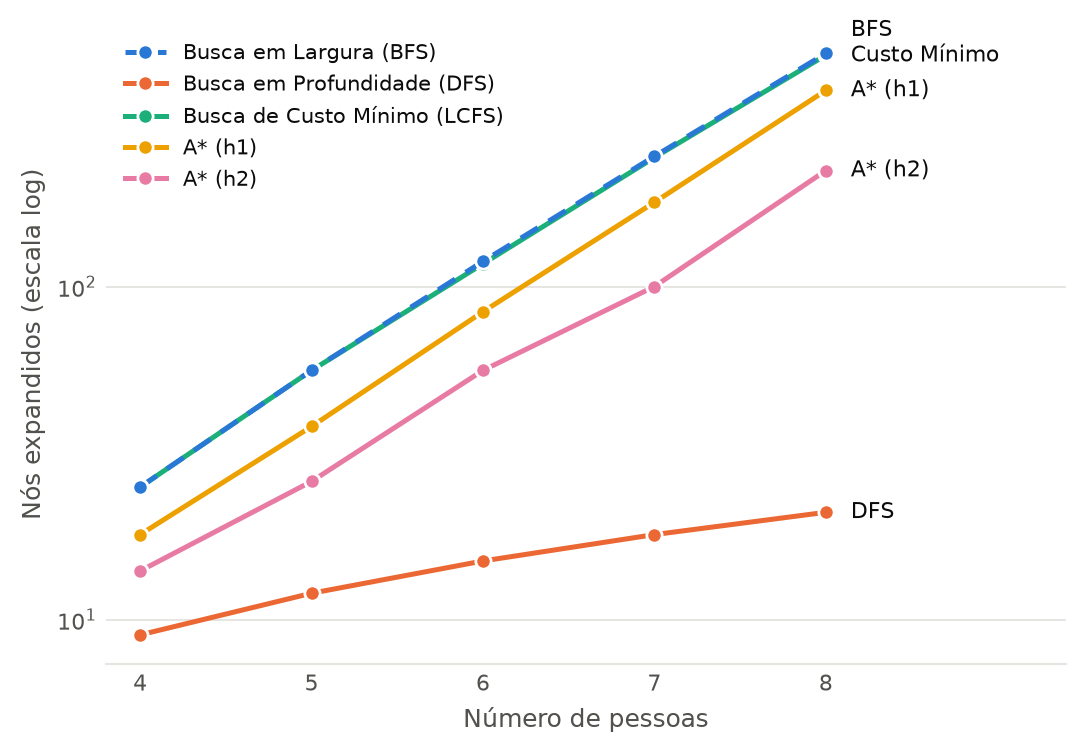
\includegraphics[width=0.85\textwidth]{escalabilidade_nos.png}
  \caption{Nós expandidos em função do número de pessoas (escala logarítmica). BFS e busca de custo mínimo praticamente coincidem: ambas varrem quase todo o grafo. Gerada por \texttt{make charts} a partir da Tabela~\ref{tab:escalabilidade}.}
  \label{fig:escalabilidade-nos}
\end{figure}

\begin{figure}[H]
  \centering
  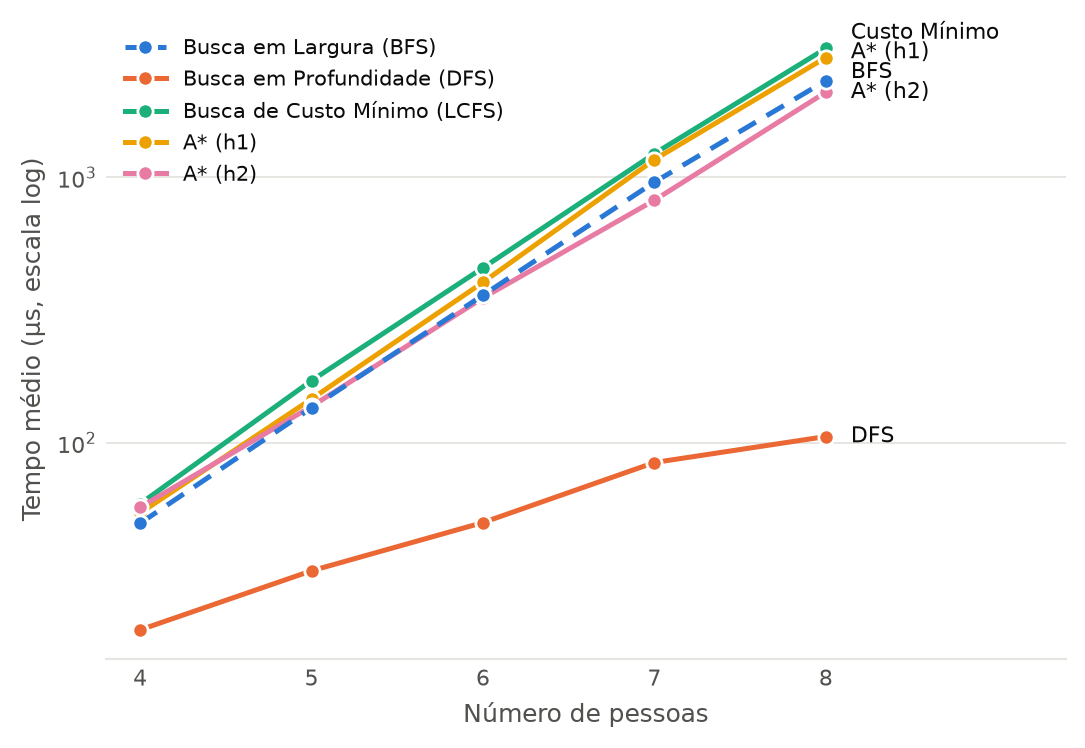
\includegraphics[width=0.85\textwidth]{escalabilidade_tempo.png}
  \caption{Tempo médio de processamento em função do número de pessoas (escala logarítmica).}
  \label{fig:escalabilidade-tempo}
\end{figure}

% TODO grupo:
%  - Motivação: com 4 pessoas o grafo tem 30 estados e tudo termina em
%    microssegundos; as diferenças entre os métodos só aparecem quando o
%    espaço cresce (2^n x 2 estados).
%  - Com 8 pessoas: custo mínimo expande 495 dos 510 estados; A*(h2) expande
%    223 (45% disso) e chega ao mesmo ótimo (Figura \ref{fig:escalabilidade-nos}).
%  - BFS e DFS: subótimos em todas as instâncias. DFS é o que menos expande e
%    nunca acerta - expandir pouco não é qualidade.
%  - Tempos (Figura \ref{fig:escalabilidade-tempo}): de h1 para h2 os nós
%    caem 42,5% em n=8, mas o tempo cai 26%: h2 custa mais por nó (ordena os
%    tempos da margem esquerda), h1 só toma um máximo. Ganho em nós não vira
%    ganho integral em tempo.
%  - Se quiserem: relação entre |V|, |E| e nós expandidos (a busca cega tende
%    a |V|).

\subsection{Limitações e possíveis extensões}
\label{sec:limitacoes}
% TODO grupo (opcional): heurísticas mais fortes (por exemplo, considerar o
% segundo mais rápido nas voltas), busca bidirecional, medição em outra
% máquina/linguagem, instâncias com capacidade 3 (a suíte de testes já cobre
% a admissibilidade de h2 nesse caso).

% -----------------------------------------------------------------------------
\section{Conclusão}
\label{sec:conclusao}
% TODO grupo: retomar as quatro tarefas e os resultados centrais em um ou dois
% parágrafos; o que o grupo aprendeu sobre a diferença entre "menos arestas" e
% "menor custo", e sobre o valor de uma heurística admissível e informativa.

% -----------------------------------------------------------------------------
\bibliographystyle{apalike}
\bibliography{referencias}

\end{document}
